\documentclass{ximera}

\author{Anna Davis} \title{MTH 140 Homework 6} 

\begin{document}

\begin{abstract}

\end{abstract}
\maketitle
 \textit{Certificate due: 10/12/2020 at 11:59 p.m.}
 
 \begin{problem}\label{prob:140hom6prob1}
 Based on meteorological daily data from the past ten years, the average of daily high temperature in Columbus, OH is 63.7 degrees Fahrenheit, with standard deviation of 20.3 degrees. 
 
 According to the Central Limit Theorem...
     \begin{multipleChoice}  
\choice{It is possible to find the probability that five daily highs selected at random will have an average of above 65 degrees.}  
\choice{The standard deviation for the distribution of sample means for samples of size 10 is $\sigma_{\overline{x}}=\frac{20.3}{\sqrt{10}}$}  
\choice{If a sample of 60 consecutive days is chosen, the average temperature for the sample will be within 5 degrees of 63.7.}  
\choice{All of the above.}  
\choice[correct] {None of the above.}
\end{multipleChoice}

 \end{problem}
 
 \begin{problem}\label{prob:140hom6prob2}
 Based on the data for 2015-17 graduates, the mean ACT Reading score was 21.4 with standard deviation of 6.5.  A sample of 100 Reading scores is chosen at random.  
 Summary of given info:
$$\sigma=\answer{6.5}$$
$$\overline{x}=\answer{21.4}$$
$$n=\answer{100}$$

\begin{center}  
\geogebra{emwxhga2}{800}{600}  
\end{center}
\begin{enumerate}
\item
What is the probability that the sample mean score is above 23?  (Use GeoGebra.  Enter your answer to four decimal places.)
$$\answer{0.0069}$$
\item What is the probability that the sample mean falls between 20 and 21?
$$\answer{0.2535}$$
\end{enumerate}
\end{problem}

\begin{problem}\label{prob:140hom6prob3}
The histogram below shows the distribution of average daily wind speeds measured at John Glenn International Airport in Columbus OH.
\begin{image}
   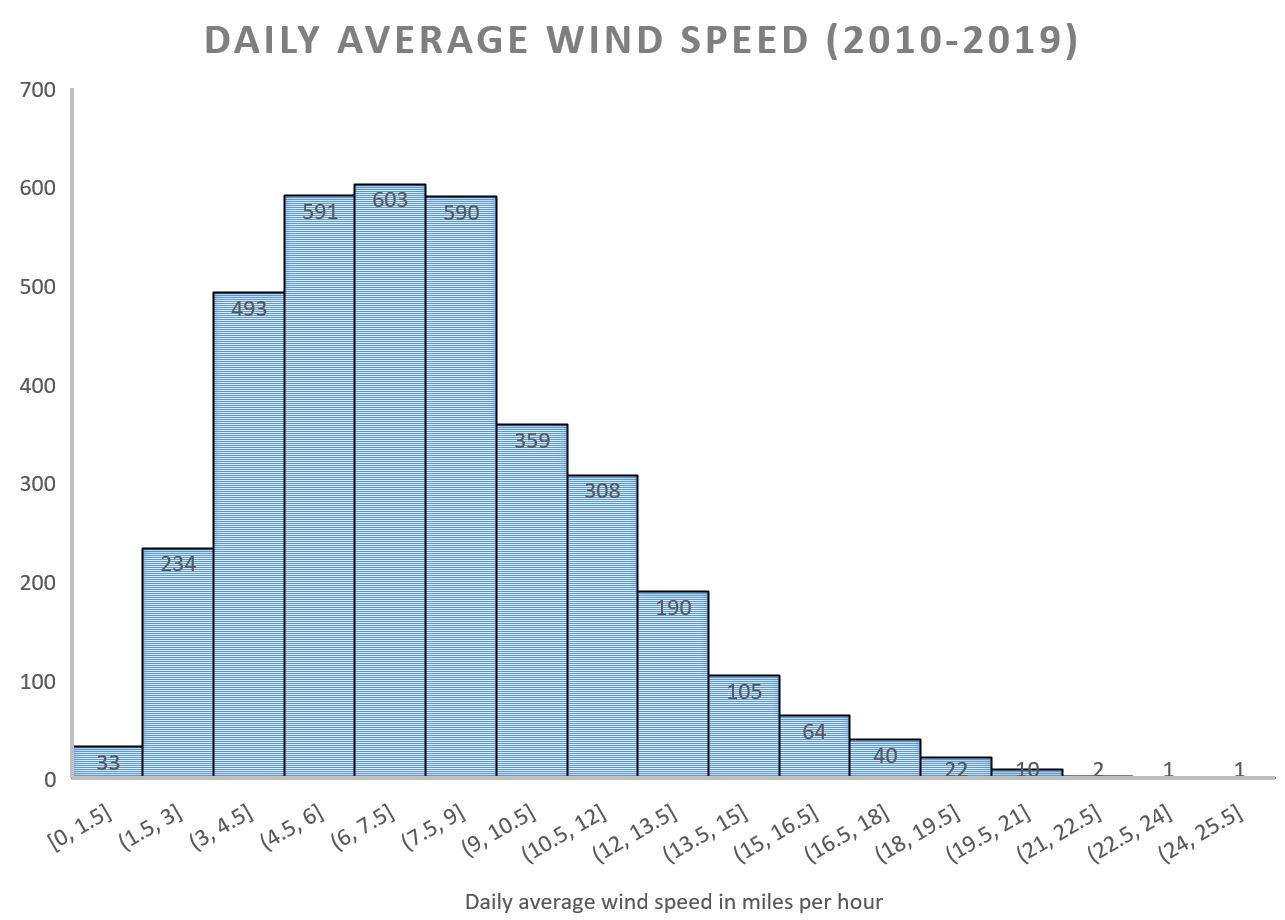
\includegraphics[height=1in]{140H6pic1.jpg}
 \end{image}
 The mean of the daily averages was found to be $\mu=7.6$ with standard deviation of $\sigma=3.6$.
 
 Answer each of the following questions using the Central Limit Theorem, IF POSSIBLE.  If the answer is impossible to find using the Central Limit Theorem, type NA into the answer box. (Case sensitive.)  Otherwise, use GeoGebra and enter your answers to four decimal places.
 \begin{enumerate}
     \item What is the probability that the average wind speed on a randomly chosen day is below 8 miles per hour?
     $$\answer{NA}$$
     \item What is the probability that a randomly selected sample of 36 days will yield a mean of less than 7.2?
     $$\answer{0.2525}$$
     \item What is the probability that the mean of daily averages for July of 2017 exceeds 8 miles per hour?
     $$\answer{NA}$$
     
 \end{enumerate}
\end{problem}
 
\begin{problem}\label{prob:140hom6prob4}
Suppose exam scores are normally distributed with an unknown population mean and a population standard deviation of 10 points. A random sample of 120 scores is taken and gives a sample mean of 72. Follow the indicated steps to find a 98\% confidence interval for the true (population) mean of exam scores.

Summary of given info:
$$\sigma=\answer{10}$$
$$\overline{x}=\answer{72}$$
$$n=\answer{120}$$
Use the Critical $z$-value table in your lecture notes to find $z_{\alpha/2}$
$$z_{\alpha/2}=\answer{2.33}$$
Error Bound for the Mean:
$$EBM=\answer{2.33}\frac{\answer{10}}{\answer[tolerance=0.01]{\sqrt{120}}}=\answer[tolerance=0.01]{2.127}$$
(Keep all significant digits in your calculator as you are doing the problem.  Round your entries to 3 decimal places.)

The 98\% confidence interval is:
$$(\answer[tolerance=0.05]{69.873},\answer[tolerance=0.05]{74.127})$$
\end{problem}

\begin{problem}\label{prob:140hom6prob5}
A machine that fills juice bottles at a factory is supposed to pour 24 fl.oz. into each bottle.  It is known from past experiments that the distribution of fill amounts is normal with a standard deviation of 0.21 fl.oz. A simple random sample of 9 bottles is tested and the sample mean amount is found to be 23.9 fl.oz.  Construct a 95\% confidence interval for the fill amount. 

Summary of given info:
$$\sigma=\answer{0.21}$$
$$\overline{x}=\answer{23.9}$$
$$n=\answer{9}$$
Use the Critical $z$-value table in your lecture notes to find $z_{\alpha/2}$
$$z_{\alpha/2}=\answer{1.96}$$
Error Bound for the Mean:
$$EBM=\answer{1.96}\frac{\answer{0.21}}{\answer{3}}=\answer{0.1372}$$
(Keep all significant digits in your calculator as you are doing the problem.  Enter your answer to 4 decimal places.)

The 95\% confidence interval is:
$$(\answer{23.7628},\answer{24.0372})$$

Assuming that 24 fl.oz. is the true mean for the fill amounts, how likely was the factory to get a sample of nine bottles with a mean of 23.9 fl.oz. or less?  Use GeoGebra to find your answer.  Enter your answer to four decimal points.
\begin{center}  
\geogebra{emwxhga2}{800}{600}  
\end{center}
$$\answer{0.0766}$$
\end{problem}
\end{document}